% These packages are optional, depending whether you want the features they provide.
% See the LaTeX Companion or other references for full information.
% !TEX TS-program = pdflatex
% !TEX encoding = UTF-8 Unicode

% This is a simple template for a LaTeX document using the "article" class.
% See "book", "report", "letter" for other types of document.

\documentclass[12pt]{article} % use larger type; default would be 10pt
\usepackage[T2A]{fontenc}
\usepackage[utf8]{inputenc} % set input encoding (not needed with XeLaTeX)
\usepackage[russian]{babel}
%%% Examples of Article customizations
% These packages are optional, depending whether you want the features they provide.
% See the LaTeX Companion or other references for full information.

%%% PAGE DIMENSIONS
\usepackage{geometry}

\usepackage{fancyhdr} 
\geometry{a4paper} % or letterpaper (US) or a5paper or....
% \geometry{margin=2in} % for example, change the margins to 2 inches all round
% \geometry{landscape} % set up the page for landscape
%   read geometry.pdf for detailed page layout information
\usepackage{sectsty}
\usepackage{graphicx} % support the \includegraphics command and options
\usepackage{mathtext}
\usepackage{amsmath}
\usepackage{amsfonts}
% \usepackage[indentfill]{indentskip} % Activate to begin indentagraphs with an empty line rather than an indent
\usepackage{biblatex}
\usepackage{hyperref}
\hypersetup{
  colorlinks=true,
  linkcolor=blue,
  urlcolor=green
}
%%% END Article customizations

%%% The "real" document content comes below...
\usepackage{setspace}
\usepackage[section]{minted}

%%% ToC (table of contents) APPEARANCE
\usepackage[nottoc,notlof,notlot]{tocbibind} % Put the bibliography in the ToC
\usepackage[titles,subfigure]{tocloft} % Alter the style of the Table of Contents

%\date{} % Activate to display a given date or no date (if empty),
         % otherwise the current date is printed 
\usepackage{physics}
\usepackage{float}
\begin{titlepage}
	\thispagestyle{empty}
	\begin{center}
	\large{МИНОБРНАУКИ РОССИИ}\\
	\footnotesize{ФЕДЕРАЛЬНОЕ ГОСУДАРСТВЕННОЕ БЮДЖЕТНОE ОБРАЗОВАТЕЛЬНОЕ УЧРЕЖДЕНИЕ}\\ 
	\footnotesize{ВЫСШЕГО ПРОФЕССИОНАЛЬНОГО ОБРАЗОВАНИЯ}\\ 
	\small{\textbf{«САНКТ-ПЕТЕРБУРГСКИЙ ГОСУДАРСТВЕННЫЙ ПОЛИТЕХНИЧЕСКИЙ УНИВЕРСИТЕТ ПЕТРА ВЕЛИКОГО»}}\\
	\hfill \break
	\normalsize{Институт компьютерных наук и технологий}\\
	\hfill \break
	\normalsize{Высшая школа искусственного интеллекта}\\
	\hfill\break
	\begin{center}
		\normalsize{Дисциплина: \\ФУНКЦИОНАЛЬНОЕ ПРОГРАММИРОВАНИЕ}
	\end{center}
	\hfill \break
	\hfill \break
	\large{ПРАКТИЧЕСКОЕ ЗАДАНИЕ 1}\\
	\hfill \break
	\hfill \break
	\hfill \break
	\hfill \break
	\hfill \break
	\hfill \break
\end{center}	

\normalsize{ 
	\begin{tabular}{ccc}
		Обучающийся &  гр. 3530201/10001 & Нгуен Куок Дат \\\\
		Руководитель & \hrulefill 				& Моторин Дмитрий Евгеньевич\\\\
	\end{tabular}
}\\
\hfill \break
\hfill \break
\hfill \break
\hfill \break
\begin{center} Санкт-Петербург 2022 
\end{center}
\end{titlepage}
\usepackage{indentfirst}
\begin{document}
\begin{center}
\input{titlepage}
\end{center}
\doublespacing
\tableofcontents
\newpage
\section{Реализация}
\subsection{Задание 1}
\textit{
	Реализовать функцию 
\[ \prod_{l=1}^{n}\sum_{k=1}^{l}\prod_{p=1}^{k}\sum_{i=1}^{p}i \]
со значением $n = 3$.}

\textit{
При запуске функции используя команду “:set +s”, записывать в отчет время выполнения и количество затрачиваемой памяти.
}

Надо реализовать 4 рекурсивных функций: сложение до $p$ \textbf{addp: Int->Int}, умножение до $k$ \textbf{mulk:Int ->Int}, сложение до $l$ \textbf{addl: Int->Int}, умножение до $n$ \textbf{muln:Int->Int}. Результат задания - вывод функции \textbf{muln}


\inputminted[firstline= 8, lastline = 22, frame=single]{Haskell}{F:/git/FuncProg/Assignment1/Assign1.hs}
\subsection{Задание 2}

\textit{
Реализовать функцию, разворачивающую список S1 = \\ \textbf{[kiveydewhjusgofiimbbyhwbopvuplwfexresmhtnic]} ([1,2,3] -> [3,2,1]).
}

Реализуют функцию \textbf{reverse1: String->String}, в которой рекурсивно перемещают голово строки в концу. 

\inputminted[firstline = 29, lastline = 31, frame= single]{Haskell}{F:/git/FuncProg/Assignment1/Assign1.hs}

\subsection{Задание 3}

\textit{
Реализовать функцию конкатенации списка списков S2 =\textbf{[[kiv], [eydew], [hjusg], [mbbyhwbopvupl], [ofii], [wfexresmhtnic]]} ([[1], [2], [3], [4]] -> [1,2,3,4])
}

Реализуют функцию \textbf{concat1: [String]->String}, в которой рекурсивно добавляют каждую данную строку в одную другую.

\inputminted[firstline = 36, lastline = 38, frame= single]{Haskell}{F:/git/FuncProg/Assignment1/Assign1.hs}

\subsection{Задание 4}

\textit{
Реализовать функцию, которая вставляет строку “-,-” между списками S2. 
}

Реализуют функцию \textbf{separate: [String] -> String}, в которой рекурсивно конкатенируют в порядке элементарную строку, $"-,-"$ в начало результатой строки. 

\inputminted[firstline = 41, lastline = 43, frame= single]{Haskell}{F:/git/FuncProg/Assignment1/Assign1.hs}

\newpage
\subsection{Задание 5}

\textit{
Реализовать вычисление элемента треугольника Паскаля (расчет i-ого числа в j-ой строке).
}
\begin{figure}[H]
\centering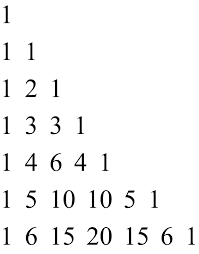
\includegraphics{pascal.png}
\caption{Треугольник Паскаля}
\end{figure}
Формула вычисления число Паскаля на строку \textbf{j} и столбец \textbf{i}:
\[ \begin{align}& p(0,0) = p (0,i) = p (i,i) = 1 \\
 & p(i,j) = p(i-1,j-1) + p(i,j -1)\end{align}\]
Реализуют функцию \textbf{pascal: (Int,Int)->Int}, в которой рекурсивно вычисляют число Паскаля с данным положением. 

\newpage
\inputminted[firstline = 48, lastline = 53, frame= single]{Haskell}{F:/git/FuncProg/Assignment1/Assign1.hs}

\subsection{Задание 5}
\subsubsection{Математическое описание}
Фракта́л 
\textit{
Реализовать вычисление элемента треугольника Паскаля (расчет i-ого числа в j-ой строке).
}
\begin{figure}[H]
\centering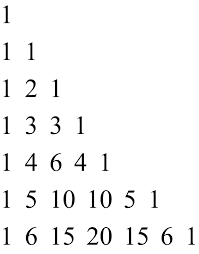
\includegraphics{pascal.png}
\caption{Треугольник Паскаля}
\end{figure}
Формула вычисления число Паскаля на строку \textbf{j} и столбец \textbf{i}:
\[ \begin{align}& p(0,0) = p (0,i) = p (i,i) = 1 \\
 & p(i,j) = p(i-1,j-1) + p(i,j -1)\end{align}\]
Реализуют функцию \textbf{pascal: (Int,Int)->Int}, в которой рекурсивно вычисляют число Паскаля с данным положением. 

\newpage
\inputminted[firstline = 48, lastline = 53, frame= single]{Haskell}{F:/git/FuncProg/Assignment1/Assign1.hs}


\end{document}